\chapter{Testing}

\begin{table}[tbhp]\centering
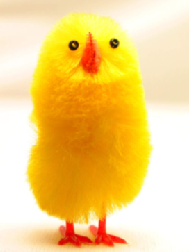
\includegraphics{chick}
\caption{A chick!}\label{chick}
\end{table}

\newcommand\explain[1]{\texttt{\meaning#1}}

\ifclasstoggle{timestamp}{\draftname}{}

\section{Another thing}\label{thing}

Click here: \url{http://www.example.com}, you should have a look at \cref{intro}, \cref{chick}, \autoref{chick}, \cref{thing}, and $\pi = 3.141592\dots$, you should know that.

%\sectionname
%\sectionautorefname

\explain\captionsspanish

\explain\extrasspanish

\makeatletter
\explain\HyLang@spanish
\makeatother
